\subsection{Style is a distribution of features}
\label{sec:Style is a distribution of features}
\textit{Style is a distribution of features} is a paper written by Eddie Huang et al. \cite{Huang:2} And bases itself on an idea in which the title describes, that style is a distribution of features. In the paper they hypothesize that the style loss in a neural transfer, when style is interpreted as a distribution of features,  would have better results by using the wasserstein metric.
\subsubsection{Wasserstein distance}
We can describe the Wasserstein distance as the minimum amount of work needed to move one distribution of mass to a target location. In this case the two distributions are the features extracted from VGG-19 layers for the generated image and the style image.\newline
The definition of the Wasserstein distance between two distributions \textit{p} and \textit{q} is: \newline
\begin{equation}
\mathcal{W}(p, q) = \inf_{\gamma \in \Gamma(p, q)} E_{x, y~\gamma}[d(x, y)]
\end{equation}
\newline
d(x, y) is any distance function, in our case squared distance $(x - y)^2$. $\Gamma(p, q)$ is the set of all joint probability distributions for \textit{p} and \textit{q}. A visual representation of a joint distribution $\gamma$ would look like this:\newline
\begin{figure}[!ht]
\begin{center}
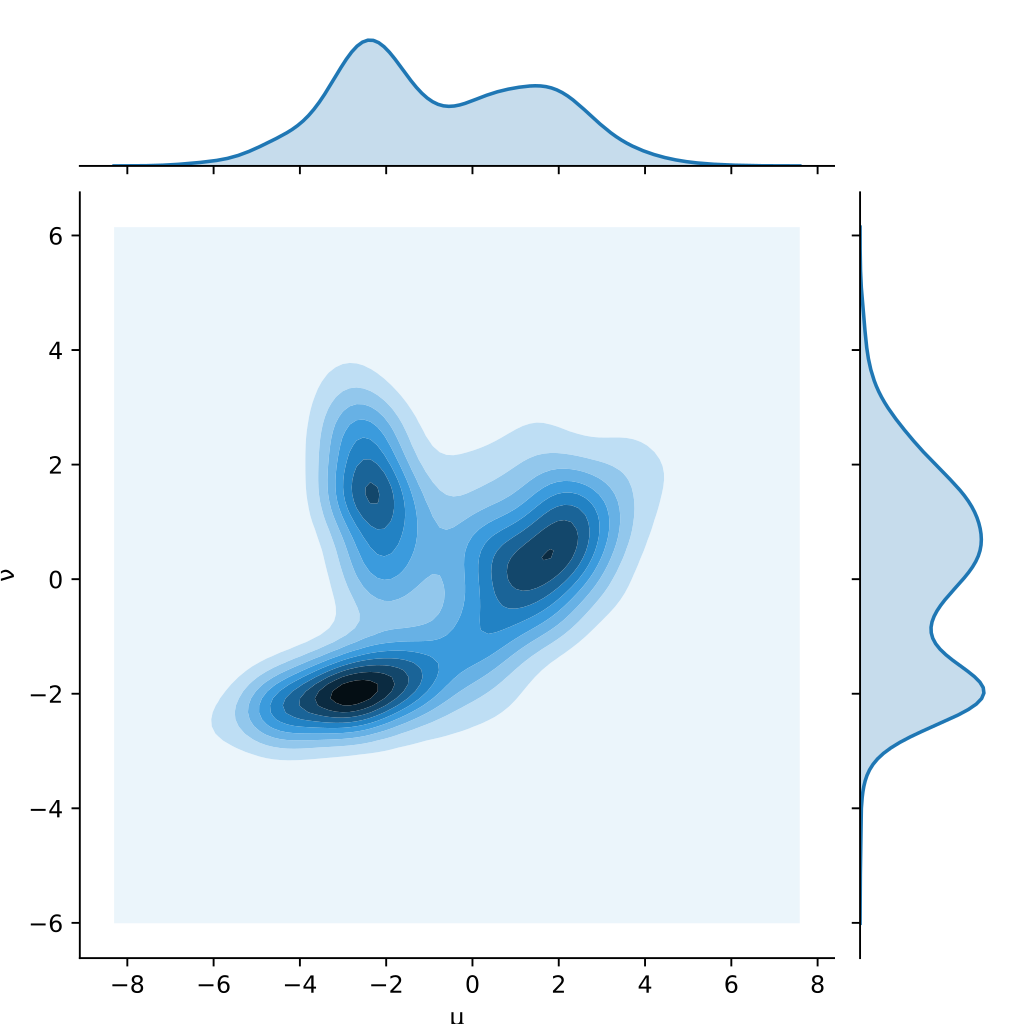
\includegraphics[scale=0.30]{report/Background/images/1024px-Transport-plan.svg.png}
\caption{A visual representation of a joint distribution}
\label{fig:featuremap}
\end{center}
\end{figure}
$\Gamma(p, q)$ contains all joint distributions $\gamma$.$ E_{x, y \text{~}\gamma}[d(x, y)]$ denotes the expected value of the variable $d(x, y)$.
\newline
By using this method of calculating the difference between the features of each layer between the generated image and the style image, the results look more convincing than the results from using the traditional style loss function from the paper by Gatys et al.\cite{Gatys:1}.\newline\newline
The drawback here is that this method is more compute-heavy than the style-loss described in the previous paper by Gatys et al. \cite{Gatys:1}.